\documentclass[a4paper,12pt]{article} 


\usepackage[T2A]{fontenc}			% кодировка
\usepackage[utf8]{inputenc}			% кодировка исходного текста
\usepackage[english,russian]{babel}	% локализация и переносы
\usepackage{amsmath, amsfonts}				% русские символы в формулах

% Математика
\usepackage{amsmath,amsfonts,amssymb,amsthm,mathtools} 

\usepackage{gensymb}	
\usepackage{wasysym}

% Картинки
\usepackage{graphicx}
\graphicspath{{images/}}

%Заговолок
\usepackage[left=2cm,right=2cm,
    top=2cm,bottom=2cm,bindingoffset=0cm]{geometry}

\usepackage{titling}


\author{Петров Артём Антонович, группа 721}
\title{"Лабораторная работа № 2.2.3 "Определение теплопроводности газов при атмосферном давлении"}
\date{\today}

\begin{document} % начало документа

\begin{minipage}[t][8cm]{\textwidth}
\maketitle
\end{minipage}


\textbf{Цель работы:} определение коэффициента теплопроводности воздуха (или $ CO_2 $) при атмосферном давлении и разных температурах.
\bigskip

\textbf{Оборудование:} прибор для определения теплопроводности; форвакуумный насос; газгольдер с углекислым газом; манометр; магазин сопротивлений; вольтметр; эталонное сопротивление в 10 Ом; источник питания.
\bigskip

\textbf{Теория}
\bigskip

Из теории известно уравнение для зависимости полного потока тепла $Q=qs$ от нити расположенной по центру соосного с ней цилиндра к стенкам этого цилиндра:

\begin{equation} \label{eq-useless}
Q = \chi \frac{2 \pi L (T_1 - T_2)}{ln \frac{r_2}{r_1}}
\end{equation}


где $r_1$ - радиус нити, $r_2$ - радиус внешнего цилиндра, $L$ - высота цилиндра, $T_1$ и $T_2$ температуры нити и цилиндра (она же температура термостата) соответственно, $\chi$ - коэффициент теплопроводности.

Из него можно получить:

\begin{equation} \label{eq-basic}
\chi = \frac{Q}{T_1 - T_2} \frac{1}{2 \pi L} ln\frac{r_2}{r_1}
\end{equation}


Основная проблема заключается в том, что не все величины, входящие в правую часть этого выражения можно непосредственно измерить использую привычные способы измерения. Для решения этой проблемы проведём сделаем небольшие преобразования:

\begin{equation} \label{eq-basic1}
Q = \frac{\chi(T_1 - T_2) 2 \pi L}{ln\frac{r_2}{r_1}}
\end{equation}

В нашем эксперименте $T_2$ поддерживается постоянной во время измерений. Значит,

\begin{equation} \label{eq-basic2}
\frac{dQ}{dT_1} = \frac{\chi 2 \pi L}{ln\frac{r_2}{r_1}} 
\end{equation}

\begin{equation} \label{eq-basic3}
\chi = \frac{dQ}{dT_1} \frac{1}{2 \pi L} ln\frac{r_2}{r_1}
\end{equation}

Также известно, что $R = R_0( 1 + \alpha T_1)$. 

\begin{equation} \label{eq-basicfinal}
\chi = \frac{dQ}{dR} \frac{dR}{dT} \frac{1}{2 \pi L} ln\frac{r_2}{r_1}
\end{equation}

Этой формулой и будем пользоваться в нашей задаче.

Также можно исследовать, как зависит $\chi$ от $T$. Из теории известно, что $\chi = AT^\beta$. D нашей работе мы найдём коэффициент $\beta$.

\bigskip

\textbf{Установка и метод измерения $\chi$:}
\bigskip

\begin{figure}[ht]
\centering
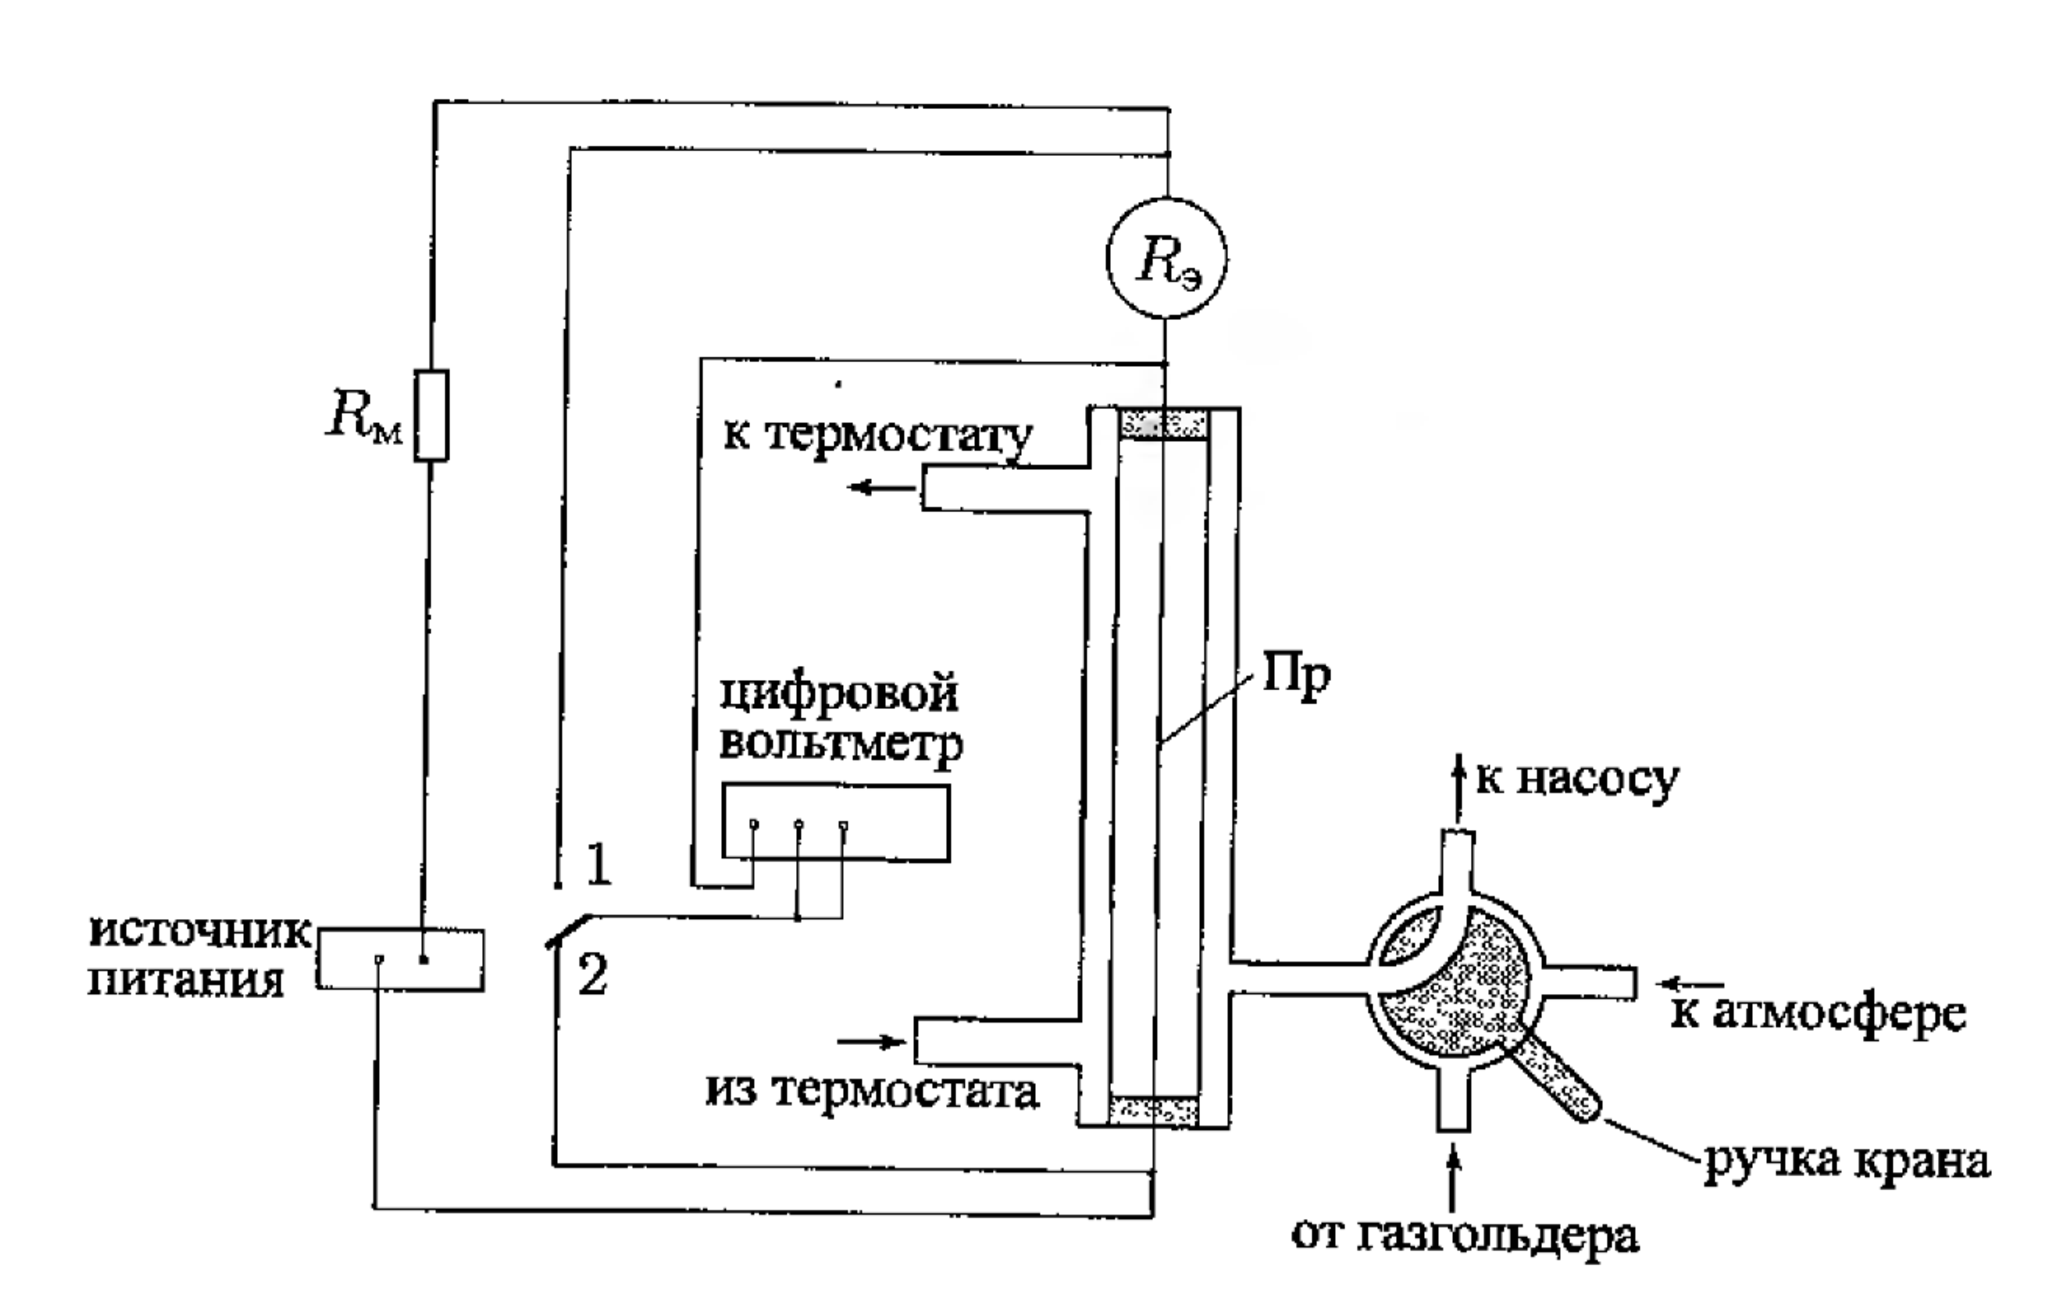
\includegraphics[width=180mm]{schema1.eps}
\caption{Схема установки для измерения теплопроводности газа.}\label{schema}
\end{figure}

Схема установки приведена на рисунке \ref{schema}. 

Значения $r_1$, $r_2$ и $L$ являются параметрами установки и легко измеряемы.  

$T_2$ определяется температурой воды в термостате. $T_1$ определяется по сопротивлению проволоки. 

Количество теплоты протекающей через газ посредством теплопроводности равно количеству теплоты, выделяющемуся в нити, если допустить, что теплота, уносящаяся за счет излучения и потери через торцы цилиндра малы. Тогда можно принять $Q = UI $. $U$ измеряется напрямую, а ток можно найти измеряя напряжение на последовательно подключенном эталонном резисторе: $I = U_\text{э} / R_\text{э} $.

Получить зависимость $R(T)$ напрямую (измеряя $R$ при разных $T_1$) с приемлемой точностью не представляется возможным так как при больших токах проволока нагревается, а при малых слишком велики термоэлектрические эффекты. Поэтому мы будем снимать зависимость $U(U_\text{э})$ и по ней строить зависимости мощности выделяющейся в нити $UU_\text{э}/R_\text{э}$ от её сопротивления $R = R_\text{э} U/U_\text{э}$ и с помощью экстраполяции находить сопротивление при нулевой протекающей мощности (а значит при температуре проволоки равной температуре термостата $T_2$). Также по этой зависимости можно найти коэффициент $\frac{dQ}{dR}$ для данной $T_2$.

Подставив полученные значения в \ref{eq-basicfinal} найдём $\chi$.

\bigskip

\textbf{Ход работы:}
\bigskip

1) Снимем зависимость $U(U_\text{э})$ при комнатной температуре. При этом важно давать системе достаточно времени для установления теплового равновесия. Для проверки этого условия после последовательного повышения $U_\text{э}$ снимем несколько точек на понижении и проверим, совпадают ли они. Также важно не допустить протекания чрезмерных токов через проволоку при измерениях, так как это может привести к её повреждению. (В нашем опыте это примерно 50-150 мА для никеля и 10-80 мА для вольфрама)

2) Повторим пункт 1 для разных значений температур.

3) Проведём анализ по описанной выше схеме. Также можно сравнить полученное значение $\alpha$ с табличным для проверки качества измерений.

4) Найдём значение $\chi$ при разных температурах. Оценим его погрешность.


\bigskip

\textbf{Записи из журнала:}
\bigskip

В работе использовались следующие приборы:

1) Вольтметр цифровой. Погрешность 0.00001\% как цена деления.

2) Термометр встроенный в термостат. Погрешность $0,1\deg C$ как цена деления.

3) Эталонное сопротивление. Погрешность 0,05 Ом как половина последней значащей цифры.

\begin{figure}[ht]
\centering
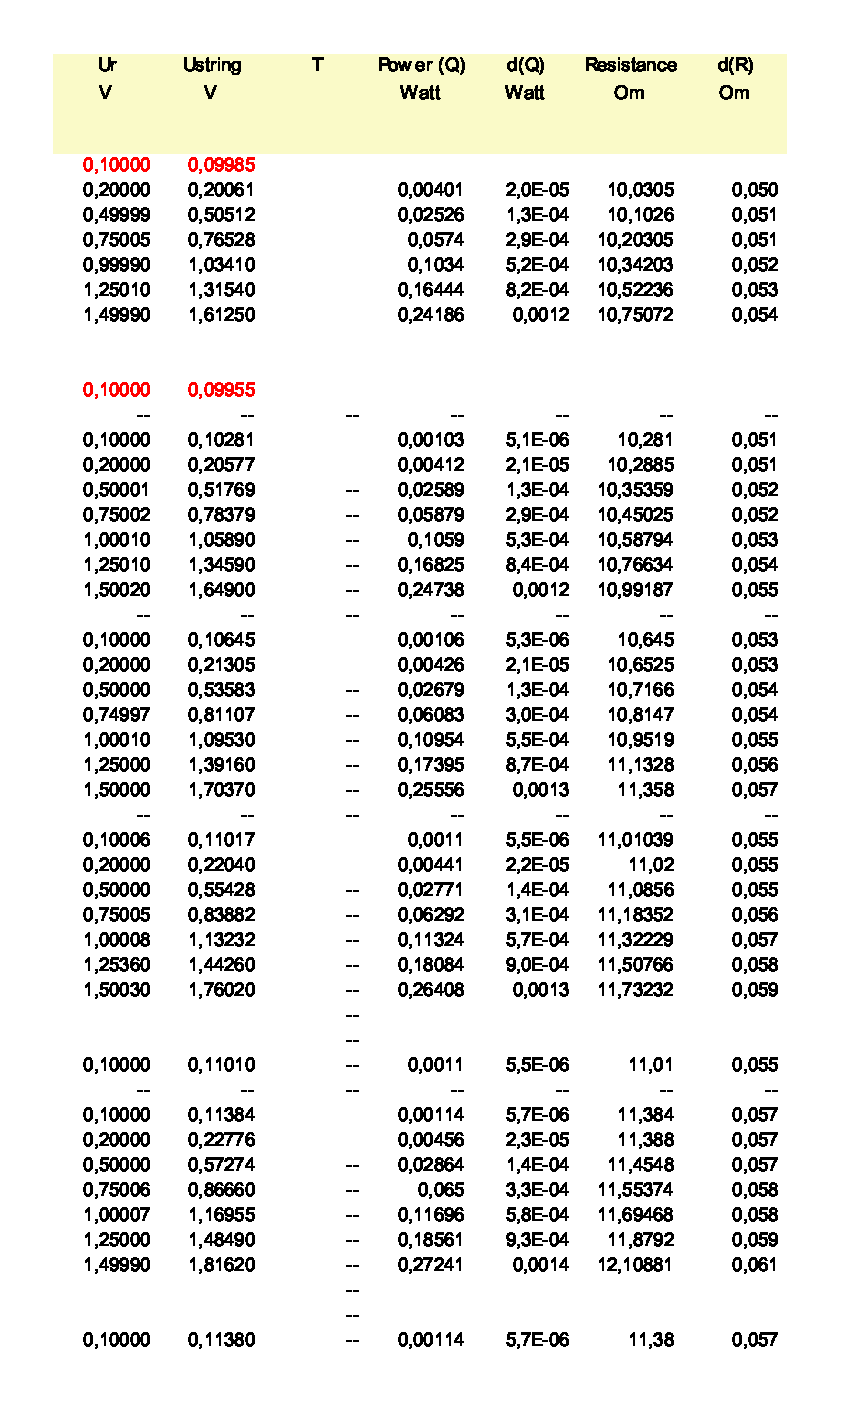
\includegraphics[width=140mm]{table0.eps}
\caption{Зависимость $U(U_\text{э})$ при разных $T_2$ (температурах термостата)}
\label{table-all}
\end{figure}

\begin{figure}[ht]
\centering
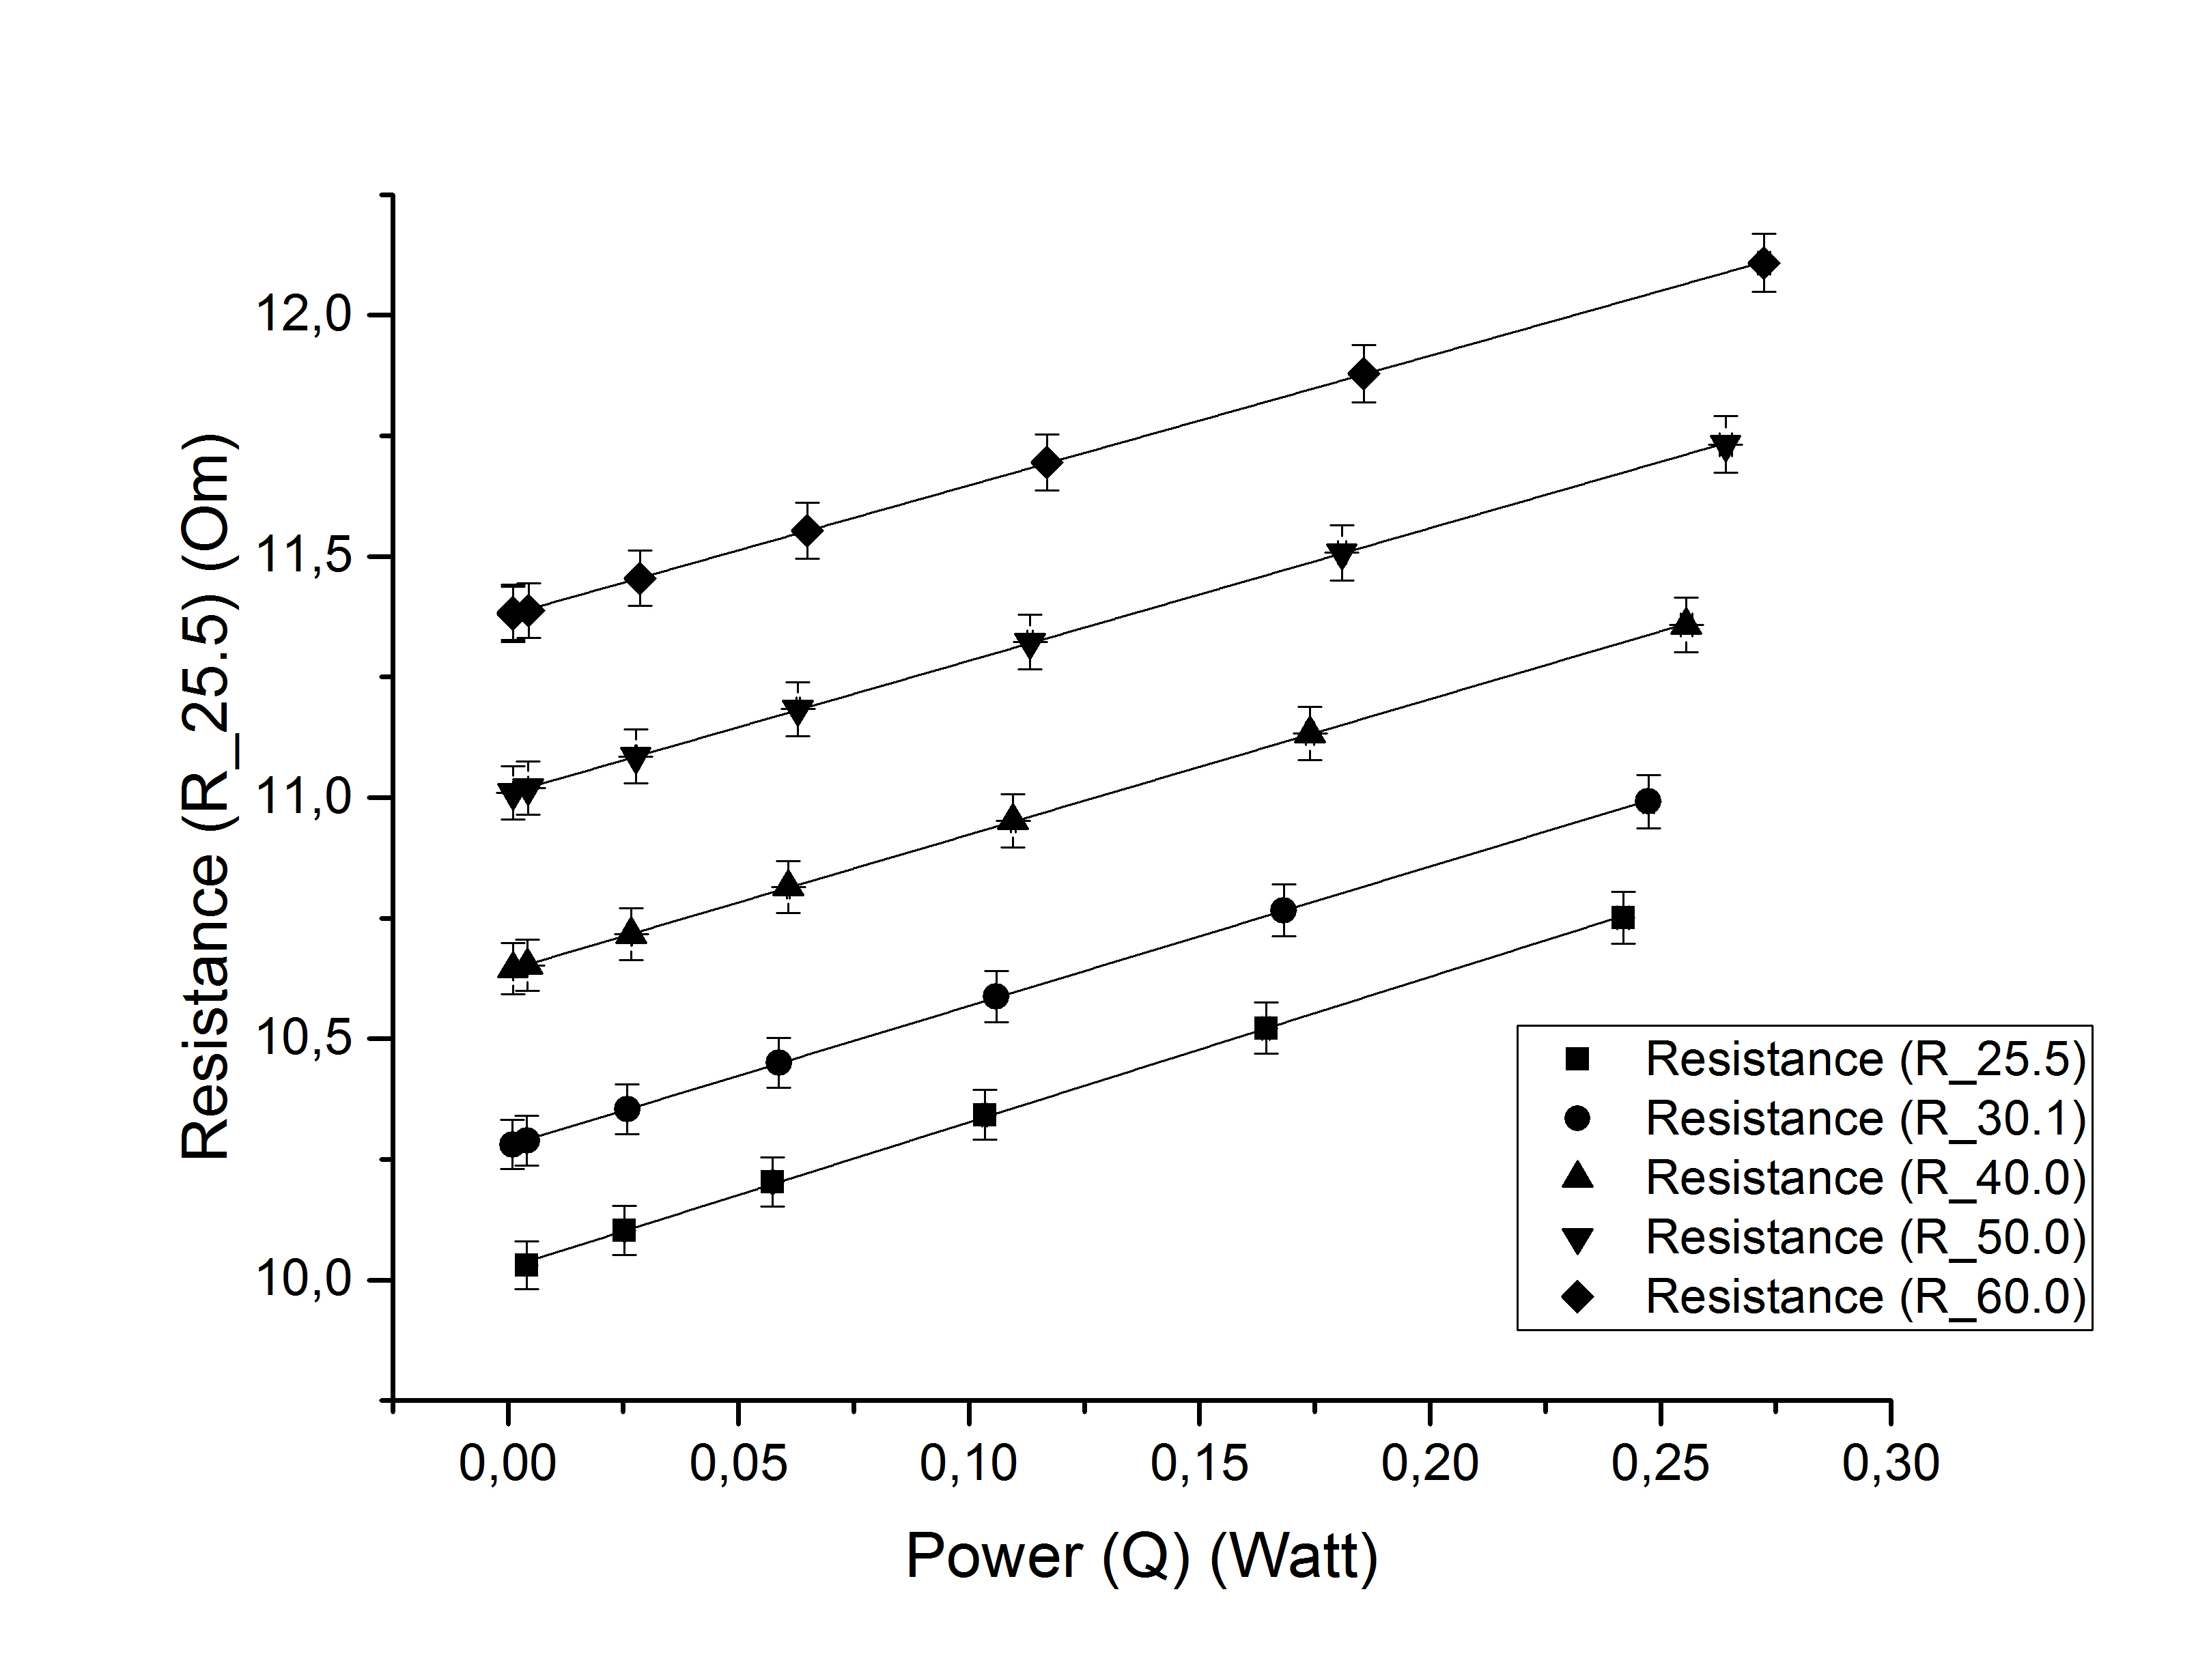
\includegraphics[width=160mm]{graph1.jpg}
\caption{График зависимости выделяемой мощности от сопротивления проволоки при разных температурах термостата ($T_2$)}
\label{graph-all}
\end{figure}

\begin{figure}[ht]
\centering
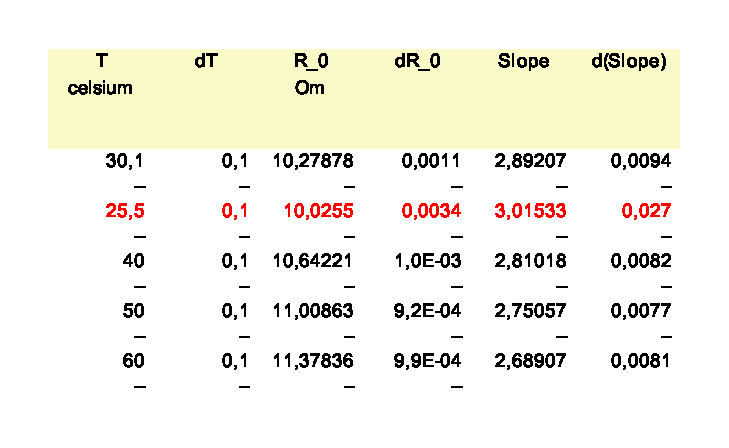
\includegraphics[width=140mm]{table3.eps}
\caption{Параметры зависимостей представленных на графике \ref{graph-all}}
\label{table-R0}
\end{figure}

Результаты полученных зависимостей $U(U_\text{э})$ при разных T представлены в таблице \ref{table-all}. Там же видны результаты обработки полученных данных.

На графике \ref{graph-all} представлены полученные зависимости $Q(R)$. Результаты их аппроксимации представлены в таблице \ref{table-R0}.

Можно заметить, что зависимость, снятая при комнатной температуре, а соответственно и при выключенном термостате несколько отличается от прочих своим наклоном и нехарактерным поведением вблизи 0 (по Q). Точки, выпадающие из линейной зависимости были исключены для более точного нахождения параметра $R_0$ - сопротивления при нулевой мощности.
Возможно, это объясняется несколько другим характером теплоотвода в данной системе из-за отключённого термостата.

Полученное среднее значение $\frac{dQ}{dR}$ (поле Slope в таблице \ref{table-R_0}) равно $2,78 \pm 0,09 $ Вт/Ом.

\begin{figure}[ht]
\centering
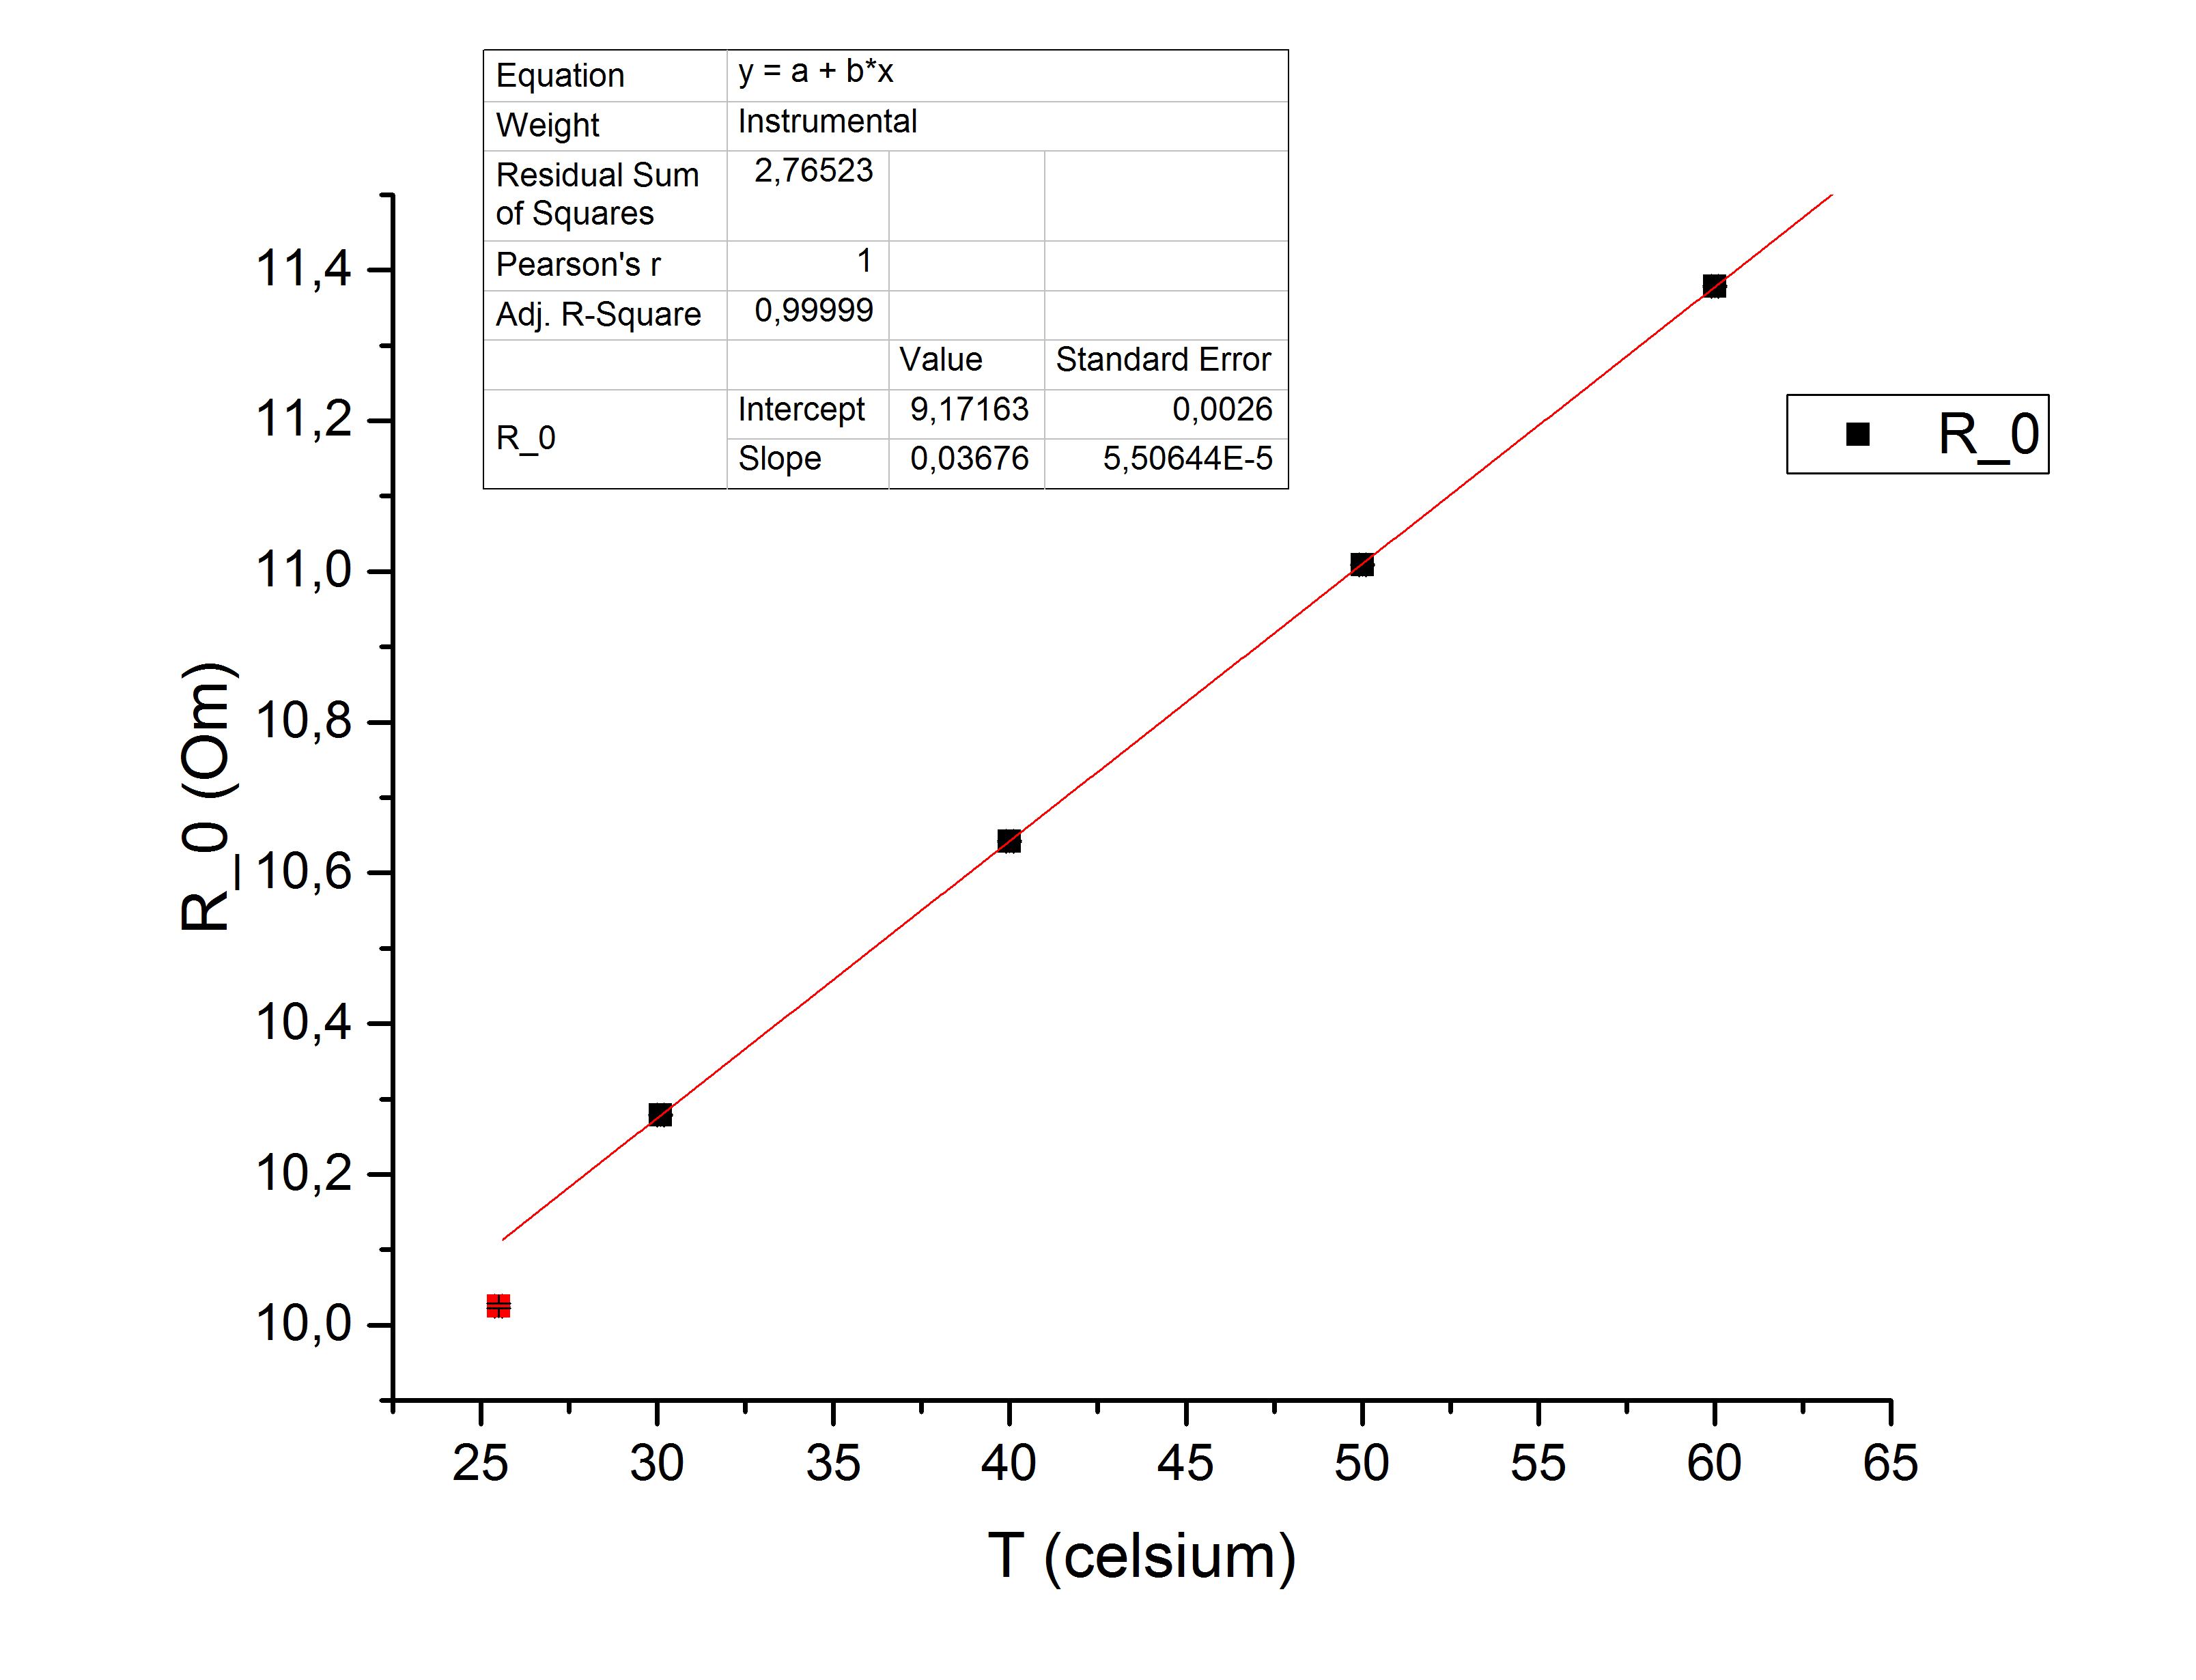
\includegraphics[width=160mm]{graph2.jpg}
\caption{График зависимости $R(T)$}
\label{graph-R0}
\end{figure} 

По полученным значениям $R_0$ найдём зависимость $R(T)$ (см. график \ref{graph-R0})  и по ней найдём $\frac{dR}{dT}$. Получено значение \underline{                 }

 что при собственно значении $R_0 \approx 10 $Ом хорошо сходится с табличным значением для меди или вольфрама.
 
По полученным данным рассчитаем $\chi$:
\bigskip

 
\end{document} % конец документа